% -*- program: xelatex -*-

\documentclass[10pt
	]{beamer}

% -----------------------------------------------------------------------------
% theming
\usetheme[numbering=fraction,
	progressbar=frametitle,
	% background=dark
	]{metropolis}


% % use a heavier font for large room/underpowered projector
% \setsansfont[BoldFont={Fira Sans SemiBold}]{Fira Sans Book}

% % can use every beamer color theme!
% \usecolortheme{crane}
% \useoutertheme{metropolis}
% \useinnertheme{metropolis}
% \usefonttheme{metropolis}

% % or set colors by hand
\definecolor{myblue}{rgb}{0.008, 0.302, 0.357}
\setbeamercolor{frametitle}{bg=myblue}
% \setbeamercolor{...}{fg=...,bg=...}
% \setbeamercolor{progress bar}{...}
% \setbeamercolor{title separator}{...}
% \setbeamercolor{progress bar in head/foot}{...}
% \setbeamercolor{progress bar in section page}{...}

% change width of title separator, section page separator % progress
%https://github.com/matze/mtheme/issues/237
\makeatletter
\setlength{\metropolis@titleseparator@linewidth}{1pt}
\setlength{\metropolis@progressonsectionpage@linewidth}{1.5pt}
\setlength{\metropolis@progressinheadfoot@linewidth}{1.5pt}
\makeatother

% -----------------------------------------------------------------------------
% do not count appendix slides, use \appendix to indicate 
\usepackage{appendixnumberbeamer}  
% creative commons icons
\usepackage[scale=2
	]{ccicons} 
% fontawesome font/icons
\usepackage{fontspec}
\usepackage{fontawesome}      %
\usepackage{pifont}
% Graphics
\usepackage{graphicx}
\usepackage{tikz}
\usetikzlibrary{shapes, arrows, positioning, calc, arrows.meta}
\usepackage{adjustbox}

% use speaker notes
\usepackage{pgfpages}
\setbeameroption{hide notes} % Only slides
%\setbeameroption{show only notes} % Only notes
% \setbeameroption{show notes on second screen=right} % Both




%%% ---------------------------------------------------------------------------
\title{Statistical Eco(-toxico)logy}
\subtitle{Improving the Utilisation of Data for\\Environmental Risk Assessment}
\date{25\textsuperscript{th} January 2017}
\author{Eduard Sz\"{o}cs}



%%% ---------------------------------------------------------------------------
\begin{document}

%%% ------------------------------
\maketitle

\begin{frame}{Table of contents}
  \setbeamertemplate{section in toc}[sections numbered]
  \tableofcontents[hideallsubsections]
\end{frame}

%%% ---------------------------------------------------------------------------
\section{Environmental Risk Assessment and Monitoring}

\begin{frame}
\frametitle{Environmental Risk Assessment and Monitoring}
 \resizebox{11.5cm}{!}{%
				% -*- root: ../../talk.tex -*-

% Define elements
% arrows, see also http://tex.stackexchange.com/questions/5461/is-it-possible-to-change-the-size-of-an-arrowhead-in-tikz-pgf/161238#161238
\tikzstyle{line} = [draw, -{Latex[length=4mm,width=3mm]}, ultra thick]
% rectangles
\tikzstyle{block} = [rectangle, draw, 
    text width=5em, text centered, rounded corners, minimum height=4em]
% papers
\definecolor{myalert}{rgb}{0.922, 0.506, 0.106}
\tikzstyle{paper} = [circle, draw, fill=myalert,  font = \bf\LARGE, minimum width=1.5cm]
\tikzstyle{textbf} = [text centered, font = \bf\Large]

% http://tex.stackexchange.com/questions/55806/mindmap-tikzpicture-in-beamer-reveal-step-by-step/55849#55849
% overlays etc in tikz
\tikzset{
    invisible/.style={opacity=0},
    visible on/.style={alt={#1{}{invisible}}},
    alt/.code args={<#1>#2#3}{%
      \alt<#1>{\pgfkeysalso{#2}}{\pgfkeysalso{#3}} % \pgfkeysalso doesn't change the path
    },
  }

 \definecolor{ao}{rgb}{0.00, 0.40, 0.60}

\begin{tikzpicture}[node distance = 2cm, auto]
	
% clip figure
\clip(-1.5,-11.5) rectangle (22.6,5);

% % % % grid for coordinates for clip
% \draw[help lines,xstep=1,ystep=1] (-2,-13) grid (30,6.5);
% \foreach \x in {-2,-1,...,30} { \node [anchor=north] at (\x,0) {\x}; }
% \foreach \y in {-13,-12,...,6} { \node [anchor=east] at (0,\y) {\y}; }


% Nodes
	%% Effects
	\node [name = exp, block, minimum width=2cm, 
		visible on=<4->] {Experiment} ;
	\node [name = stat, block, minimum width=2cm, right=1cm of exp,
	visible on=<4-7>] {Data / Statistics} ;
	\node [name = stat, block, minimum width=2cm, right=1cm of exp, color=myalert, 
	visible on=<8->] {Data / Statistics} ;
    \node [name = eff, block, 
		minimum width=57mm, 
		minimum height=25mm, 
		below left=5mm of exp.west, anchor = west,
	visible on=<2->] {} ;
	\node[textbf, below right=8mm and 5mm of exp, anchor = south,
	visible on=<2->]{Effects};

	%% Exposure
  	\node [name = prop, block, minimum width=2cm, below=38mm of exp, 
  	visible on=<3->] {Data / Properties} ;
	\node [name = model, block, minimum width=2cm, right=1cm of prop,
	visible on=<3->] {Models} ;
	\node [name = expo, block, 
		minimum width=57mm, 
		minimum height=25mm, 
		below = 20mm of eff,
	visible on=<2->] {} ;
	\node[textbf, above=-2mm of expo, anchor = north, , 
	visible on=<2->]{Exposure};

	%% Risk Assessment
	\node [name = risk, block, below right=0.75cm and 1cm of stat,
       minimum width=45mm, 
		minimum height=2.5cm, 
		font = \bf\large,
		align = center,
       text width = 3cm,
       visible on=<1->] {Environmental Risk\\  Assessment};

	%% Monitoring data
	\node [name = monit, block, 
		right = 9cm of risk,
        minimum width=35mm, 
		minimum height=20mm, 
		font = \bf\large,
		align = center,
        text width = 3cm,
        visible on=<1->] {Environmental\\ Monitoring};

	%% biological data
	\node [name = bio, block, 
		above left = 2cm and 2cm of monit, anchor = north,
		minimum width=30mm, align = center, text width = 30mm, font=\large,
		visible on=<5->] {Biology   };
	%% chemical data
	\node [name = chem, block, 
		below left = 2cm and 2cm of monit, anchor = south,
		minimum width=3cm, font=\large,text width = 30mm,
		visible on=<6-8>] { Chemistry};
	\node [name = chem, block, 
		below left = 2cm and 2cm of monit, anchor = south,
		minimum width=3cm, font=\large,text width = 30mm, color=myalert,
		visible on=<9->] { Chemistry};


  %% Chapters
	\node[name = chap2, paper, 
		above left = 5mm and -15mm of stat, 
		anchor = east,
		visible on=<8->]{1};	
    \node[name = chap3, paper, 
		below left = -22mm and 0mm of chem, anchor = north, 
		visible on=<9->
		]{2};
	\node[name = chap4, paper, anchor = north, yshift=-25mm,  xshift = 10mm,
		visible on=<11->] (chap4) at ($(chem)!0.5!(expo)$) {3};
	\node[name = chap5, paper, anchor = south, yshift=20mm, xshift = 10mm,
		visible on=<12->] (chap5) at ($(bio)!0.5!(eff)$) {4};
   \node[name=rl1, below= 0mm of chap4, font=\Large, color=myalert,
   visible on=<11->]{Retrieve \& Link data};
      \node[name=rl1, above= 0mm of chap5, font=\Large, color=myalert,
   visible on=<12->]{Retrieve \& Link data};

   \node[name=dir, above= 25mm of eff, font=\Large, text width = 60mm, fill = ao, text=white, xshift=10mm,
   visible on=<1->]{\textbf{Plant Protection Products 1107/2009}};
   \node[name=wfd, right= 90mm of dir, font=\Large, text width = 65mm, 
   fill = ao, text=white,
   visible on=<1->]{\textbf{Water Framework Directive 2000/60/EC}};


% papers
   	\node[name = chap2a, paper, 
		below = 45mm of expo, 
		anchor = east,
		visible on=<8>]{1};	
	\node[name = chap2t, right = 5mm of chap2a, font = \bf\Large, color = myalert, 
	visible on=<8>]{Szöcs \& Schäfer (2015). “Ecotoxicology is not normal”. ESPR 22(18), 13990–13999.};

	\node[name = chap3a, paper, 
		below = 45mm of expo, 
		anchor = east,
		visible on=<9-10>]{2};	
	\node[name = chap3t, right = 5mm of chap3a, font = \bf\Large, color = myalert, text width = 200mm,
	visible on=<9-10>]{Szöcs, Brinke, Karaoglan \& Schäfer (submitted). “Large scale risks from pesticides in small streams”. ES\&T.};

	\node[name = chap4a, paper, 
		below = 45mm of expo, 
		anchor = east,
		visible on=<11>]{3};	
	\node[name = chap4t, right = 5mm of chap4a, font = \bf\Large, color = myalert, text width = 200mm,
	visible on=<11>]{Szöcs \& Schäfer (accepted). “webchem: An R Package to Retrieve Chemical Information from the Web”. JSS.};

	\node[name = chap5a, paper, 
		below = 45mm of expo, 
		anchor = east,
		visible on=<12>]{4};	
	\node[name = chap5t, right = 5mm of chap5a, font = \bf\Large, color = myalert, text width = 200mm,
	visible on=<12>]{Chamberlain \& Szöcs (2013). “taxize: taxonomic search and retrieval in R”. F1000Research 2(191).};

% arrows
	\path [line,
	visible on=<4->] (exp) -- (stat);
	\path [line, 
	visible on=<3->] (prop) -- (model);
	\path [line,
	visible on=<4->] (eff) -| node[pos = 0.4, font = \large]{RAC} (risk);
	\path [line,
	visible on=<3->] (expo) -| node[pos = 0.4, font = \large,  below]{PEC} (risk);
	\path [line,
	visible on=<6->] (monit) |- (chem);
	\path [line,
	visible on=<5->] (monit) |- (bio);
	\path [line, dashed,
	visible on=<11->] (chap4) edge [bend left = 15, color=myalert]  (prop);
    \path [line, dashed,
    visible on=<12->] (chap5) edge [bend right = 15, color=myalert]   (stat);
	\path [line, dashed,
	visible on=<11->] (chap4) edge [bend right = 15, color=myalert]   (chem);
    \path [line, dashed,
    visible on=<12->] (chap5) edge [bend left = 15, color=myalert]   (bio);
    \path [dashed,
    visible on=<10->] ([yshift=5mm]bio.south west) edge[line, bend left = -10]   ([yshift=0mm]risk.north east);
    \path [dashed,
    visible on=<10->] (chap3.north west) edge [line, bend right = 30] node[xshift = 20mm, yshift =9mm, font = \large, align = center] {Retrospection}  (risk);
	\path [dashed,
	visible on=<7->] (risk.south east) edge [line ,bend right = 40]  node [xshift = 10mm, pos =0.2,  below, font = \large, align = center, fill = white] {Approves \\ Substance} (chem);


\end{tikzpicture}

				}
\end{frame}


%%% ---------------------------------------------------------------------------
\section{Improving Statistics in ERA}

% \begin{frame}
% \frametitle{test}
% 	\begin{itemize}
% 		\item<1-> Eggs
% 		\item<2-> Plants
% 		\note[item]<2>{Tell joke about plants.}
% 		\note[item]<2>{Make it short.}
% 		\item<3-> Animal
% 	\end{itemize}
% \end{frame}
% % this will be on a separate note:
% \note[enumerate]{\item foo \item bar \item baz \item foobar}

\begin{frame}
\frametitle{Ecotoxicology is not normal}

\end{frame}



\begin{frame}
\frametitle{A brief history of GLM (uncomprehensive)}

\end{frame}


\begin{frame}
\frametitle{Statistical Power is unacceptably low}

\end{frame}


\begin{frame}
\frametitle{Generalized Linear Models (GLM) can do better}

\end{frame}



\begin{frame}
\frametitle{What we learned}

\end{frame}


\begin{frame}
\frametitle{Where are we now?}

\end{frame}

%%% ---------------------------------------------------------------------------
\section{Exploring Monitoring Data for ERA}

\begin{frame}
\frametitle{Environmental Monitoring}

\end{frame}

\begin{frame}
\frametitle{Thresholds}

\end{frame}

\begin{frame}
\frametitle{Statistics with chemical measurements}

\end{frame}


\begin{frame}
\frametitle{Dynamics}

\end{frame}


\begin{frame}
\frametitle{Risks}

\end{frame}


\begin{frame}
\frametitle{What we learned}

\end{frame}

%%% ---------------------------------------------------------------------------
\section{Solutions for Linking Data in ERA}

\begin{frame}
\frametitle{Biologists \& Chemists face the same problems}
	\small
	\centering
	\textbf{\alert{Names}}
	\begin{columns}[t]
	\column{.45\textwidth}
	\emph{Osmia rufa, Osmia bicornis, Osmia ruffa, Osmia unilandauis, Osmia spec.} 
	\column{.45\textwidth}
	Chlorpyrifos, Chlorpyriphos, Chlorphyrifos, Chlorpyrifos-ethyl, Chlorpypifot
	\end{columns}
	\pause

	\centering
	\textbf{\alert{Hierarchies}}
	\begin{columns}[t]
	\column{.45\textwidth}
	Hymenoptera/ Apoidea/ Megachilidae/ Osmia/ rufa 
	\column{.45\textwidth}
	organophospate, ester, insecticide
	\end{columns}
	\pause

	\centering
	\textbf{\alert{Traits / Properties}}
	\begin{columns}[t]
	\column{.45\textwidth}
	Wing length, Mass, Season 
	\column{.45\textwidth}
	Mass, $K_{OW}$, $LC_{50}$
	\end{columns}
	\pause

	\centering
	\textbf{\alert{Identifiers}}
	\begin{columns}[t]
	\column{.45\textwidth}
	NCBI, ITIS, EOL, ... 
	\column{.45\textwidth}
	2921-88-2, Clc1c(OP(=S)[...], InChI=1S/C9H11C[...], SBPBAQFW[...], CSID,...
	\end{columns}
	\vspace{0.8em}
	\pause

	\rule{\textwidth}{1pt}
	\textbf{\alert{Amount of data}}

	\begin{columns}[t]
	\column{.45\textwidth}
	\centering
	2993 taxa
	\column{.45\textwidth}
	\centering
	489 pesticides \\ (+ 590 other organics)
	\end{columns}
\end{frame}


{%
\setbeamertemplate{frame footer}{Münch et al. (2016). DoOR 2.0 - Comprehensive Mapping of Drosophila melanogaster Odorant Responses. Scientific Reports 6, 21841
}
\begin{frame}{}
\frametitle{Instead of wasting time...}
... use \alert{webchem}! \\
	\hspace*{2cm}
	\begin{adjustbox}{max totalsize={\textwidth}{0.8\textheight}}
				% -*- root: ../../talk.tex -*-

\definecolor{blue}{RGB}{32, 126, 153}
\definecolor{green}{RGB}{33, 182, 78}
\definecolor{red}{RGB}{246, 72, 45}
\definecolor{orange}{RGB}{246, 146, 45}
\definecolor{yellow}{RGB}{180, 180, 18}

\begin{tikzpicture}[node distance = 0.2cm, auto]

%styles
\tikzstyle{circ} = [circle, draw, text = black,   line width=1pt, 
    text width=4cm, text centered, scale=1, font=\bf\huge]
\tikzstyle{rect} = [rectangle, draw, text = black, line width=1pt,
    text width=5cm, text centered, rounded corners, minimum height=1.5cm, minimum width=1cm, font=\bf\huge]

\tikzstyle{line} = [draw, -{Latex[length=5mm,width=3mm]}, line width=1mm, opacity = 0.8]

    % input nodes
    \node [circ, fill=green] (cas_i) {CAS};
    \node  (name_i) [circ, below=of cas_i, fill = blue] {Name};
    \node  (inchikey_i) [circ, below=of name_i, fill = red] {InChiKey};
    \node  (other_i) [circ, below=of inchikey_i, fill =orange] {Other};
   
   % source nodes
   \node (cir) [rect, right=of cas_i, shift={(13,7)}, fill = yellow]{CIR};
   \node (chemspider) [rect, below=1cm of cir, fill = yellow]{ChemSpider};
   \node (cts) [rect, below=1cm of chemspider, fill = yellow]{CTS};
   \node (etox) [rect, below=1cm of cts, fill = yellow]{ETOX};
   \node (chemid) [rect, below=1cm of etox, fill = yellow]{ChemID};
  \node (opsin) [rect, below=1cm of chemid, fill = yellow]{OPSIN};
  \node (alan) [rect, below=1cm of opsin, fill = yellow]{Pesticide Compendium};
  \node (wiki) [rect, below=1cm of alan, fill = yellow]{wikidata};
  \node (pubchem) [rect, below=1cm of wiki, fill = yellow]{PubChem};
  \node (pan) [rect, below=1cm of pubchem, fill = yellow]{PAN};
  \node (src) [rect, below=1cm of pan, fill = yellow]{SRC};

	% output nodes
    \node (cas_o) [circ, right=of cir, shift={(15,-5)}, , fill =green] {CAS};
    \node  (name_o) [circ, below=of cas_o, , fill =blue] {Name};
    \node  (inchikey_o) [circ, below=of name_o, fill =red] {InChiKey \\ InChi};
    \node  (smiles_o) [circ, below=of inchikey_o, fill =red] {SMILES};
    \node  (legis_o) [circ, below=of smiles_o, fill =orange] {Legislation};
    \node  (syno_o) [circ, below=of legis_o, fill =orange] {Synonyms};
    \node  (other_o) [circ, below=of syno_o, fill =orange] {Other};
    \node (prop_o) [circ, above=of cas_o, fill =orange] {Properties};
    \node (tox_o) [circ, above=of prop_o, fill =orange] {Toxicology};

    %paths
   % from cas_i
    \path [line, green] (cas_i.east) -- (cir.west);
    \path [line, green] (cas_i.east) -- (chemspider.west);
    \path [line, green] (cas_i.east) -- (cts.west);
    \path [line, green] (cas_i.east) -- (etox.west);
    \path [line, green] (cas_i.east) -- (chemid.west);
    \path [line, green] (cas_i.east) -- (alan.west);
    \path [line, green] (cas_i.east) -- (wiki.west);
    \path [line, green] (cas_i.east) -- (pubchem.west);
    \path [line, green] (cas_i.east) -- (pan.west);
    \path [line, green] (cas_i.east) -- (src.west);

	% from name_i
    \path [line, blue] (name_i.east) -- (cir.west);
    \path [line, blue] (name_i.east) -- (chemspider.west);
    \path [line, blue] (name_i.east) -- (cts.west);
    \path [line, blue] (name_i.east) -- (etox.west);
    \path [line, blue] (name_i.east) -- (chemid.west);
    \path [line, blue] (name_i.east) -- (opsin.west);
    \path [line, blue] (name_i.east) -- (alan.west);
    \path [line, blue] (name_i.east) -- (wiki.west);
    \path [line, blue] (name_i.east) -- (pubchem.west);
    \path [line, blue] (name_i.east) -- (pan.west);

    %from inchikey_i
    \path [line, red] (inchikey_i.east) -- (cir.west);
    \path [line, red] (inchikey_i.east) -- (chemspider.west);
    \path [line, red] (inchikey_i.east) -- (cts.west);
    \path [line, red] (inchikey_i.east) -- (chemid.west);
    \path [line, red] (inchikey_i.east) -- (wiki.west);
    \path [line, red] (inchikey_i.east) -- (pubchem.west);
   
    %from other_i
    \path [line, orange] (other_i.east) -- (cir.west);
    \path [line, orange] (other_i.east) -- (chemspider.west);
    \path [line, orange] (other_i.east) -- (cts.west);
    \path [line, orange] (other_i.east) -- (etox.west);
    \path [line, orange] (other_i.east) -- (wiki.west);
    \path [line, orange] (other_i.east) -- (pubchem.west);

   %from cir
  \path [line, orange] (cir.east) -- (prop_o.west);
  \path [line, green] (cir.east) -- (cas_o.west);
  \path [line, blue] (cir.east) -- (name_o.west);
  \path [line, red] (cir.east) -- (inchikey_o.west);
  \path [line, red] (cir.east) -- (smiles_o.west);
  \path [line, orange] (cir.east) -- (other_o.west);

  %from chemspider
  \path [line, orange] (chemspider.east) -- (prop_o.west);
  \path [line, blue] (chemspider.east) -- (name_o.west);
  \path [line, red] (chemspider.east) -- (inchikey_o.west);
  \path [line, red] (chemspider.east) -- (smiles_o.west);

  % from cts
  \path [line, blue] (cts.east) -- (name_o.west);
  \path [line, green] (cts.east) -- (cas_o.west);
  \path [line, red] (cts.east) -- (inchikey_o.west);
  \path [line, red] (cts.east) -- (smiles_o.west);
  \path [line, orange] (cts.east) -- (syno_o.west);
  \path [line, orange] (cts.east) -- (other_o.west);

	% from etox
   \path [line, orange] (etox.east) -- (tox_o.west);
   \path [line, green] (etox.east) -- (cas_o.west);
   \path [line, blue] (etox.east) -- (name_o.west);
   \path [line, orange] (etox.east) -- (legis_o.west);
   \path [line, orange] (etox.east) -- (syno_o.west);
   \path [line, orange] (etox.east) -- (other_o.west);

  %from chemid
   \path [line, orange] (chemid.east) -- (tox_o.west);
   \path [line, orange] (chemid.east) -- (prop_o.west);
   \path [line, green] (chemid.east) -- (cas_o.west);
   \path [line, blue] (chemid.east) -- (name_o.west);
   \path [line, red] (chemid.east) -- (inchikey_o.west);
   \path [line, red] (chemid.east) -- (smiles_o.west);
   \path [line, orange] (chemid.east) -- (syno_o.west);

	%from opsin
    \path [line, green] (opsin.east) -- (cas_o.west);
   \path [line, red] (opsin.east) -- (inchikey_o.west);
   \path [line, red] (opsin.east) -- (smiles_o.west);

   %from alan wood
   \path [line, green] (alan.east) -- (cas_o.west);
   \path [line, blue] (alan.east) -- (name_o.west);
   \path [line, red] (alan.east) -- (inchikey_o.west);
   \path [line, orange] (alan.east) -- (other_o.west);

  %from wiki
   \path [line, green] (wiki.east) -- (cas_o.west);
   \path [line, red] (wiki.east) -- (inchikey_o.west);
   \path [line, red] (wiki.east) -- (smiles_o.west);
   \path [line, orange] (wiki.east) -- (other_o.west);

  % from pubchem
     \path [line, orange] (pubchem.east) -- (prop_o.west);
     \path [line, blue] (pubchem.east) -- (name_o.west);
     \path [line, red] (pubchem.east) -- (inchikey_o.west);
     \path [line, red] (pubchem.east) -- (smiles_o.west);
     \path [line, orange] (pubchem.east) -- (syno_o.west);

    % from pan
    \path [line, orange] (pan.east) -- (tox_o.west);
    \path [line, orange] (pan.east) -- (prop_o.west);
     \path [line, blue] (pan.east) -- (name_o.west);
   \path [line, green] (pan.east) -- (cas_o.west);
   \path [line, orange] (pan.east) -- (legis_o.west);
   \path [line, orange] (pan.east) -- (other_o.west);

  %from src
       \path [line, orange] (src.east) -- (tox_o.west);
     \path [line, blue] (src.east) -- (name_o.west);
   \path [line, green] (src.east) -- (cas_o.west);

\end{tikzpicture}

	\end{adjustbox}

\pause
\vspace*{-1cm}\emph{''\alert{webchem} ...likely saved hundreds of working hours''}
\end{frame}
}


{%
\setbeamertemplate{frame footer}{Dr. Susan E. Johnston, University of Edinburgh. On twitter.
}
\begin{frame}
\frametitle{Instead of wasting time...}
... use \alert{taxize!} \\
	\hspace*{-2cm}
	\begin{center}
	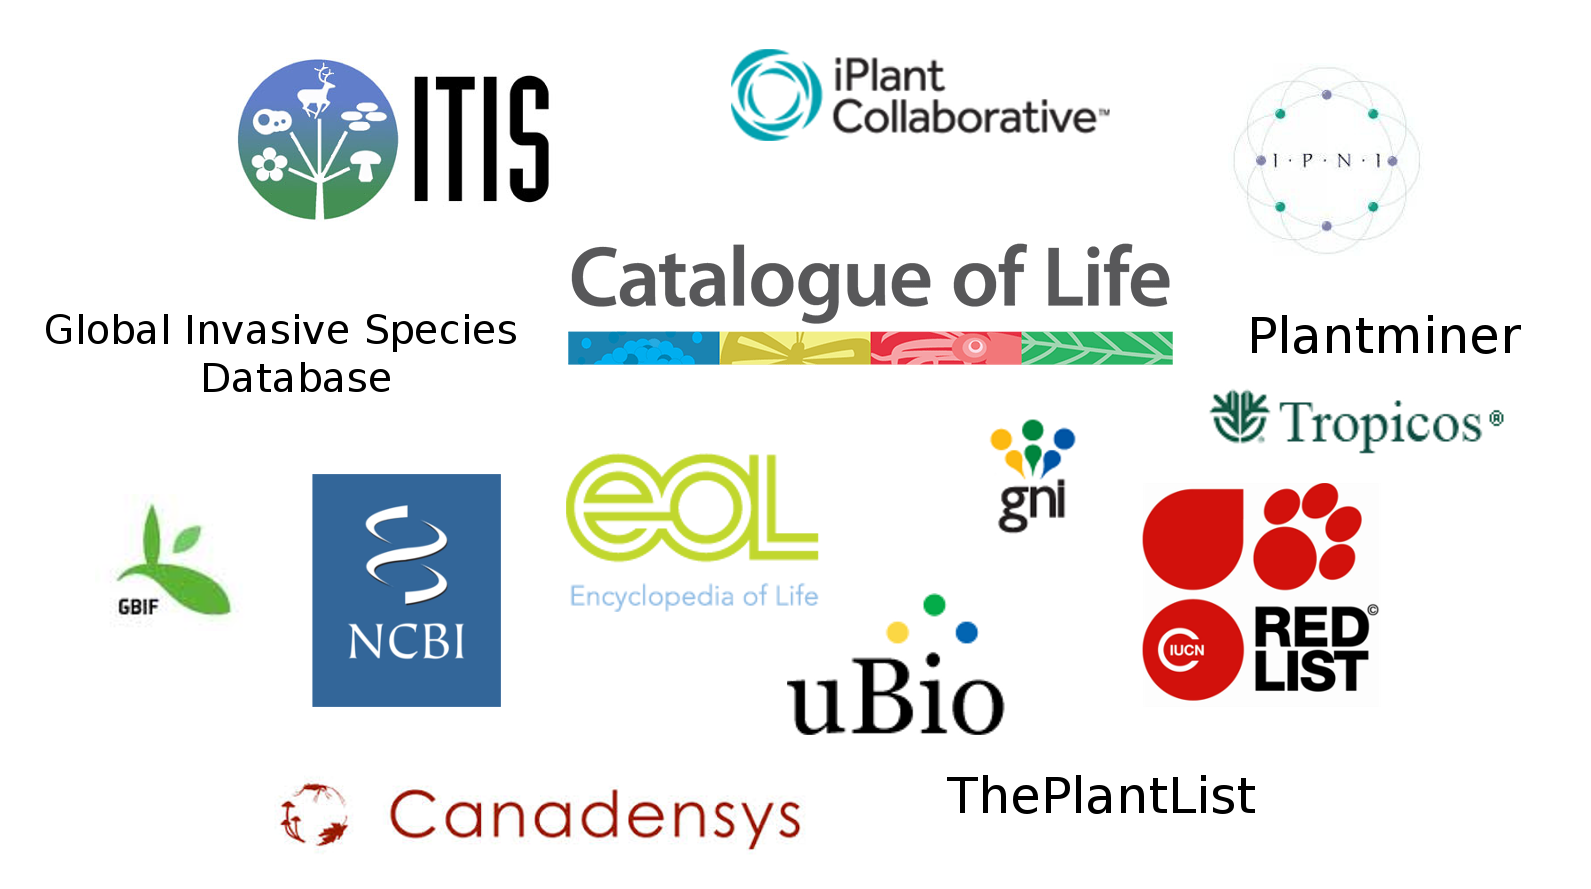
\includegraphics[height=0.6\textheight]{figs/sources_taxize.png}
	\end{center}

\pause
\emph{''Days of searching done during my morning coffee. Amazing. \alert{taxize}.''}
\end{frame}
}



%%% ---------------------------------------------------------------------------
\section*{Recap}

\begin{frame}
\frametitle{What we learned}
	\metroset{block=fill}
	\begin{exampleblock}{\checkmark Improving Statistics in ERA}
		\begin{itemize}
			\item Change your model, not your data
			\item Ultimately ban NOEC
			\item Take LOQ into account
		\end{itemize}
	\end{exampleblock}

\pause
	\begin{exampleblock}{\checkmark Exploring Monitoring Data for ERA}
		\begin{itemize}
			\item Pesticide Dynamics
			\item Agricultural small streams at risk
			\item Neonicotinoids
			\item Feedback for ERA
		\end{itemize}
	\end{exampleblock}

\pause
	\begin{exampleblock}{\checkmark Solutions for Linking Data in ERA}
		\begin{itemize}
			\item Handling big eco(toxico-)logical data not easy
			\item Now easier
		\end{itemize}
	\end{exampleblock}


\end{frame}


%%% ---------------------------------------------------------------------------
%%% Final slide
\begin{frame}[standout]
	\frametitle{}

	\vspace{1em}
	\Huge{Statistical Ecotoxicology} \\[0.3em]
	\large{Improving the Utilisation of Data for \\ Environmental Risk Assessment} \\[1em]

	\normalsize
	Eduard Szöcs \\[3em]

	\faLaptop~~~\textbf{\href{http://edild.github.io/}{http://edild.github.io/ }}\\[.5em]
	\faTwitter~~~\textbf{\href{http://twitter.com/EduardSzoecs}{@EduardSzoecs}} 	\\[0.5em]
	\faFilePowerpointO~~~\textbf{\href{https://github.com/edild/phd_defense}{https://github.com/edild/phd\_defense}}\\[0.5em]
	\faBook~~~\textbf{\href{https://github.com/edild/phd_thesis}{https://github.com/edild/phd\_thesis}}\\[3em]

	\begin{center}\ccbysa\end{center} 

\end{frame}


\appendix

\begin{frame}
\frametitle{Statistics?}

\end{frame}


\begin{frame}
\frametitle{ZAGA what...?}

\end{frame}


\begin{frame}
\frametitle{Comparison with Stehle / Knauer?}

\end{frame}

\begin{frame}
\frametitle{Mixtures => mainly one compound}

\end{frame}



\begin{frame}
\frametitle{ecology / biota?}

\end{frame}


% ------------------------------
\end{document}
